% Chapter 2

\chapter{Background} % Write in your own chapter title
\label{Chapter2}
\lhead{Chapter 2. \emph{Background and Related Work}}

\section{Related Work}

There were many research that has been done on weather classification. Most works use method - extracting features plus classifiers~\citep{bishop1995neural,roser2008classification,serrano2002computationally,gokalp2007scene}.
Some work on low-level features, like color~\citep{szummer1998indoor}, texture~\citep{shotton2009textonboost,vailaya2002automatic}. Some use filters or segmentation~\citep{boutell2004learning,shotton2009textonboost} to extract high-level features, such as sky, shadow~\citep{lutwo}. Some works use statistical measure methods~\citep{he2014spatial,roser2008classification} to analyse low-level feature distribution.

Generally, traditional methods follow three basic steps\citep{roser2008classification,yan2009weather}. First, some Regions of Interest (ROIs), for example, sky and shadow,  are extracted from a weather image. Then, histogram descriptors are used to represent the difference between them. Finally, a classifier, e.g., Support Vector Machine, is built up based on the extracted features. 

Most previous jobs are based on discriminative model. They extracted human recognizable features to classify scene. This type of shadow learning depends mainly on quality of features and human being prior knowledge. An image without prior features or poor features is hard to classify. Furthermore, the methods require a lot of work on data pre-processing and are not flexible. And the approaches depends on structural information to category a image into one of classes. Structural information is concluded from illumination invariant features, like SIFT. However, previous jobs have limits on classifying diversity images. It is hard to list total factors which determinate the weather condition.

\section{Single-Layer Networks}

Artificial neurons were introduced as information processing devices more than fifty years ago\citep{mcculloch1943logical}. Following the early work, perceptrons were deployed in layers to do pattern recognition job. A lot of resource was invested in researching capability of learning perceptrons theoretically and experimentally. As shown in Figure 2.1, a perceptron computes a weighted summation of its n inputs and then thresholds the result to give a binary output y. We can treat n input as an vector with n elements, and represent the vector as either class A(for output +1) or class B(for output -1).
\graphicspath{ {./Figures/} }
\begin{figure}[!htb]
\centering
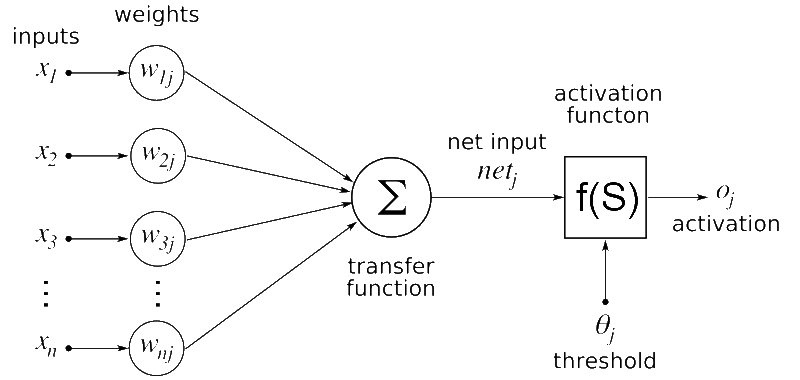
\includegraphics[width=0.8\textwidth]{Figure2-1.png}
\caption{\label{fig:perceptron}Diagram of a perceptron.}
\end{figure}

Each output is updated according to the equation:
\begin{equation}\label{eq:BasicEq}
y_{i} = f(h_{i}) = f\left(\sum_{j}w_{ij}x_{j}\right)
\end{equation}
where $y_{i}$ is the $i$th output, $h_{i}$ is the net input into node $i$, The weight $w_{ij}$ connects the $i$th output and the $j$th input, and $x_{j}$ is the $j$th input. The threshold function $f(h)$ is the activation function and usually makes up the form
\begin{equation}\label{eq:FullEq}
f(h) = sign(h) = 
  \begin{cases}
    -1       & \quad h < 0 \\
    1  & \quad h \geq 0\\
  \end{cases}
\end{equation}
and it can be plotted out
\graphicspath{ {./Figures/} }
\begin{figure}[!htb]
\centering
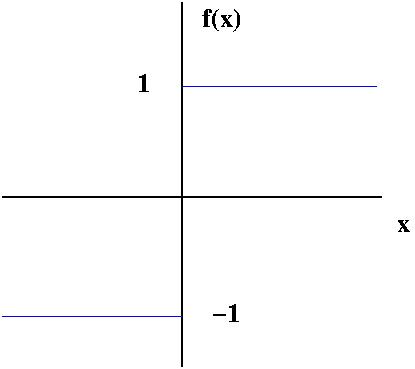
\includegraphics[width=0.4\textwidth]{bipolar-threshold.jpg}
\caption{\label{fig:1LayerErrorSurface}Threshold function}
\end{figure}

Besides threshold function, there are servel deterministic action functions.
\begin{itemize}
  \item Linear function 
\begin{equation}\label{eq:LinearFunc}
f(h) = h
\end{equation}

\graphicspath{ {./Figures/} }
\begin{figure}[!htb]
\centering
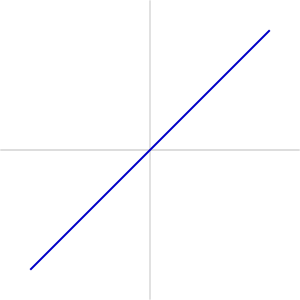
\includegraphics[width=0.4\textwidth]{Linear_function.png}
\caption{\label{fig:1LayerErrorSurface}Linear function}
\end{figure}
  
  \item Sigmoid function
\begin{equation}\label{eq:SigmoidFunc}
f(h) = \frac{1}{1+e^{-h}}
\end{equation}

\graphicspath{ {./Figures/} }
\begin{figure}[!htb]
\centering
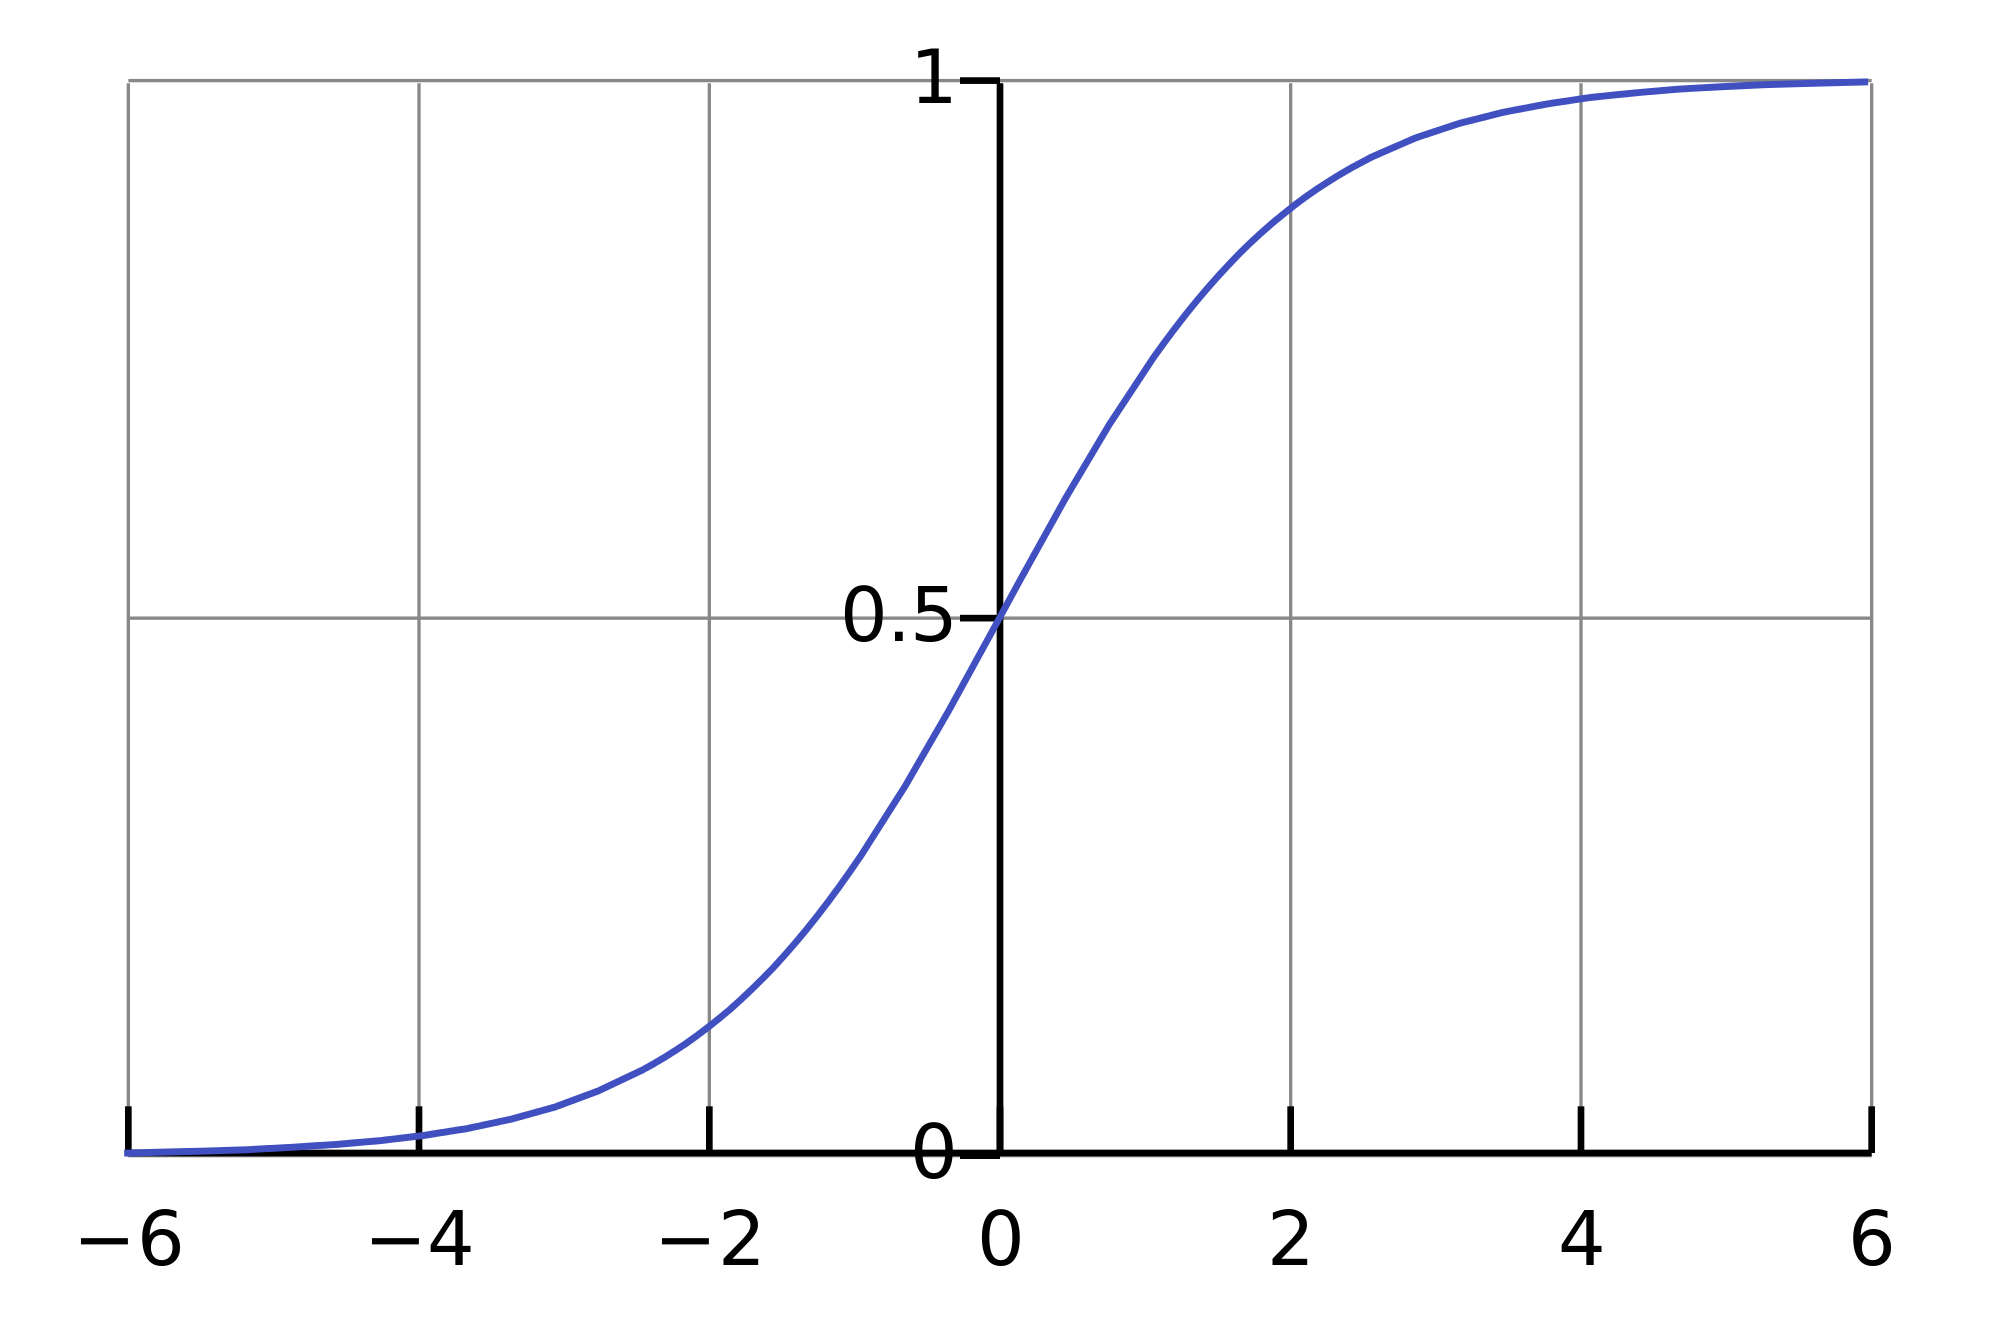
\includegraphics[width=0.4\textwidth]{Logistic-curve.png}
\caption{\label{fig:1LayerErrorSurface}Sigmoid function}
\end{figure}

  \item tanh function)
\begin{equation}\label{eq:TanhFunc}
f(h) = tanh(h)
\end{equation}

\graphicspath{ {./Figures/} }
\begin{figure}[!htb]
\centering
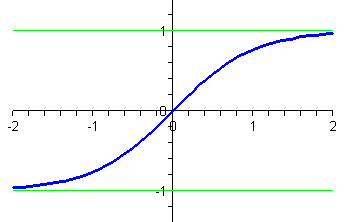
\includegraphics[width=0.4\textwidth]{tanh.png}
\caption{\label{fig:1LayerErrorSurface}Tanh function}
\end{figure}
%  \item The third etc \ldots
\end{itemize}

We can also represent \ref{eq:FullEq} in vector notation, as in 
\begin{equation}\label{eq:UsedEq}
y = f(h) = f(\bf w \cdot x)
\end{equation}
where \textbf{w} and \textbf{x} can be regarded as $nx1$ dimensional column vectors, and $n$ is the number of input data.
The term $w \cdot x$ in \ref{eq:UsedEq} constructs a $(n-1)$-dimension hyperplane which passes the origin. The hyperplane can be shifted by adding an parameter to \ref{eq:BasicEq}, for example
\begin{equation}\label{eq:WithBias}
y = f(h) = f(\bf w \cdot x + b)
\end{equation}
We can have the same effect by putting a constant value $1$ and increase the size of $x$ and $w$ by one. The extra weight $w$ with fixed value 1 is called \textit{bias weight}; it is adaptive like other weights and provides flexibility to hyperplane. Then we get:
\begin{equation}\label{eq:finalEq}
y = f(h) = f(\sum_{i=0}^{n}w_{i}x_{i})
\end{equation}
The aim of learning is to find a set of weights $w_{i}$ so that:
\begin{align*}
y = f(\sum_{i=0}^{n}w_{i}x_{i}) = 1  & \quad x \in Class A\\
y = f(\sum_{i=0}^{n}w_{i}x_{i}) = 0  & \quad x \in Class B
\end{align*}

Single layer neural network classifier is simple to implement, while it can only support a linear decision boundary. We can build a pretty simple neural network to acquire intuition behind mathematical theory. The network has no bias and one neuron which means it has one weight, say $w1$. And we implement a logistic sigmoid activation function on the multiply of input data and weight $w1$. Therefore, the network can map the input data $a_0$ onto an output $a_{out}$ based on the function
\begin{equation}\label{eq:1LayerExample}
a_{out} = f(a_{0}w_{1})
\end{equation}
where $f()$ is a logistic function. Supposing that an input data $1$ maps to an output data $1$, we can compute the value of the error function for each possible value of $w_{1}$. Feeding value of $w_{1}$ in range $(-10,10)$, we can plot error surface in Figure\ref{{fig:1LayerErrorSurface}}.
\graphicspath{ {./Figures/} }
\begin{figure}[!htb]
\centering
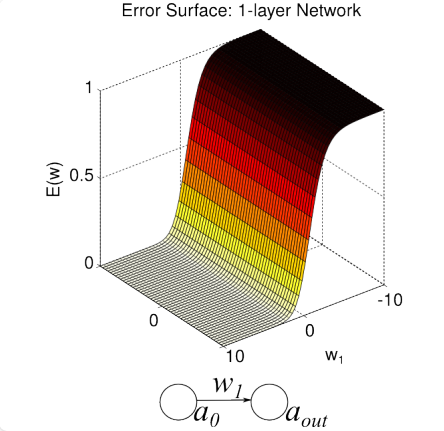
\includegraphics[width=0.4\textwidth]{1LayerErrorSurface.png}
\caption{\label{fig:1LayerErrorSurface}Error surface for a single layer neural network. Source: Internet}
\end{figure}

Single layer neural network has a decision boundary which is linear. However, it is clear this is a very limited class of decision boundary. It can be illustrated by two types of dataset.
\graphicspath{ {./Figures/} }
\begin{figure}[!htb]
\centering     %%% not \center
\subfigure{\label{fig:a}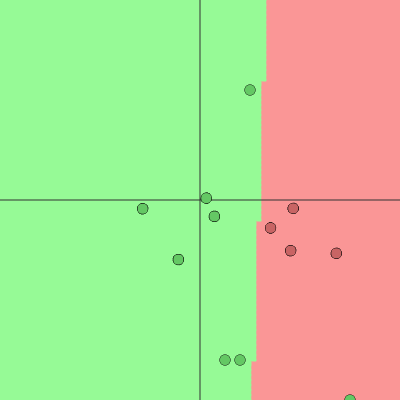
\includegraphics[width=0.4\textwidth]{SingleLayerSimpleData}}
\subfigure{\label{fig:b}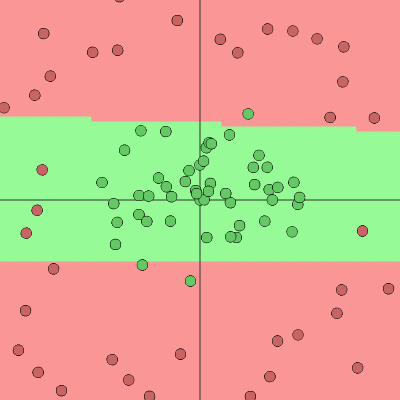
\includegraphics[width=0.4\textwidth]{SingleLayerCircleData}}
\caption{Two types of dataset. Left one can be separated by a single layer neural network. Right one cannot be separated by a single neural network.}
\end{figure}

\section{Multi-Layer Networks}

Single layer networks have some important limitation in terms of the representing range of functions. We are seeking to learn the nonlinearity as the linear discriminant.To improve the representation capability, we can stack layers networks. This is the approach of multilayer neural networks. Multilayer neural networks implement linear discriminants via mapping input data to a nonlinear space. They can use fairly simple algorithms to learn form of the nonlinearity from training data.

In the thesis, we limit multi-layer networks in subset of feedforward networks. As feedforward networks can provide a general mechanism for representing nonlinear functional mapping between a set of input data and a set of labels. The \ref{fig:ffnet} is a feedforward network having two layers of adaptive weights.

\begin{figure}[!htb]
\centering
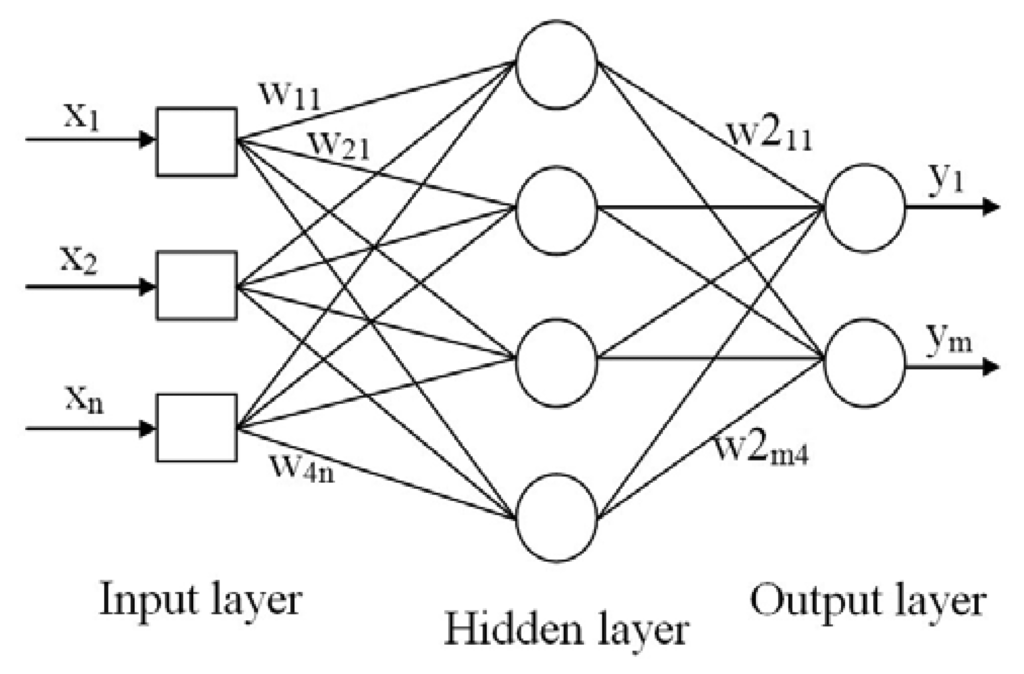
\includegraphics[width=0.8\textwidth]{Figure2-2.png}
\caption{\label{fig:ffnet}Diagram of a feedford neural networks.}
\end{figure}

In the example, the middle column perceptrons act as hidden units. The network has $n$ inputs, $4$ hidden units and $m$ output units. The network diagram represents the function in the form
\begin{equation}\label{eq:ffEq}
y_{m} = \hat{f}\Big(\sum_{j=0}^{m}w_{j4}^{(2)}f\big(\sum_{i=0}^{n}w_{4i}^{(1)}x_{i}\big)\Big)
\end{equation}
In the \ref{eq:ffEq}, outer activation function could be different with the inner one.

There are some choices for activation functions, sigmoid and tanh are related and can provide high capability with continuous input data. Logistic activation function sigmoid can be represented as 
\begin{equation}\label{eq:sigmoid}
f(x) = \frac{1}{1+e^{-x}}
\end{equation}
Its outputs lies in range $(0,1)$. We can do a linear transformation $hat{x}=x/2$ on input data and a linear transformation $hat{y}=2y-1$ on the output. Then we can get an equivalent activation function tanh which can be represented as
\begin{equation}\label{eq:tanh}
f(x) = tanh(x) = \frac{e^{x}-e^{-x}}{e^{x}+e^{-x}}
\end{equation}

The three layer neural network is capable of approximating any function with enough hidden units which means the networks with two layers of weights and sigmoid nonlinearities can provide any accuracy in classification problems. 

Again, we can use a simple example to illustrate the power of multilayer neural network. In this example, we have one input, one hidden neuron and one output. There is no bias in input layer and hidden layer. There are two weights existing in the network, say $(w_{1}, w_{2})$, and the output can be calculated via
\begin{equation}\label{eq:2LayerExample}
a_{out} = f(f(a_{0}w_{1})w_{2})
\end{equation}
where $f()$ is logistic function. With varying $w_{1}$ and $w_{2}$, the error surface can be represented
\graphicspath{ {./Figures/} }
\begin{figure}[!htb]
\centering
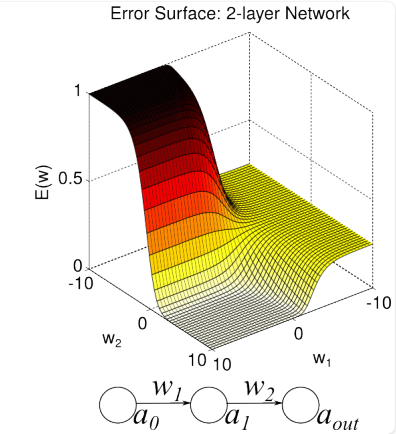
\includegraphics[width=0.4\textwidth]{2LayerErrorSurface.png}
\caption{\label{fig:2LayerErrorSurface}Error surface for a multilayer neural network. Source: Internet}
\end{figure}
And the samples which cannot be separated by single neural network can be done by multilayer neural network.
\graphicspath{ {./Figures/} }
\begin{figure}[!htb]
\centering
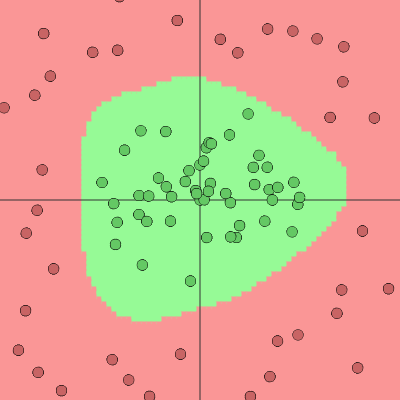
\includegraphics[width=0.4\textwidth]{MultiLayerCircleData.png}
\caption{\label{fig:2LayerErrorSurface}A multilayer neural network can separate a complicated dataset. Source: Internet}
\end{figure}

\section{Stochastic Gradient Descent}

Because weights space in neural networks is continuous, training can reach the optimal weights value through optimization algorithms, which means minimizing loss value of function
\begin{equation}\label{eq:LossMin}
L(f_{w}) = \sum L(y, f_{w}(x))
\end{equation}
Gradient descent is a method which starts from a random point, then moves to a nearby point that is downhill repeatly. It converges on a minimum possible loss.

Stochastic gradient descent is a subtype of gradient descent. It only considers a single training point and move to nearby point based on
\begin{equation}\label{eq:SGDUpdate}
w = w - \eta  \Delta L(w) = w - \eta \sum_{i=1}^{n} \Delta L_{i}(w)
\end{equation}
where $\eta$ is the learning rate and $L_{i}(w)$ is the value of the loss function at the $i^{th}$ sample. Although stochastic gradient descent does not guarantee convergence, it is fast.

\section{Backpropagation}

Multi-layer neural networks can represent mapping from input data to output classes. How to learn a suitable mapping from training dataset? And there is no explicit mapping between output and hidden units. This will be resolved by a popular learning algorithm-backpropagation.

Because networks have differentiable activation functions, the activation of output units can be propagated to hidden units with regard to weights and bias. If we have an error function, we can evaluate derivatives of the error and update the weights to minimize the error function via some optimization methods.

Backpropagation can be applied to find the derivatives of an error function related to the weights and biases in the network via two stages. First, the derivatives of the error functions, for instance sum-of-squares and Jacobian, with respect to the weights must be evaluated. Second, a variety of optimization schemes can be implemented to compute the adjustment of weights based on derivatives. After putting data forward propagation through the network, we can get the output result. It updates weight changes based on grandient descent. Suppose the network has $i$ inputs, $h$ hidden units and $k$ outputs. The update equation can be represented as 
\begin{equation}\label{eq:UpdateWeights}
w(j+1) = w(j) + \Delta w(j)
\end{equation}
where $\Delta w(j)$ defined as 
\begin{equation}\label{eq:DeltaWeights}
\Delta w(j) = -\eta \frac{\partial E}{\partial w}
\end{equation}

For the hidden to output layer weights
\begin{equation}\label{eq:h2oBP}
\Delta w(jk) = -\eta \frac{\partial E}{\partial w_{jk}} = -\eta \delta_{k}y_{j}
\end{equation}
where $$\delta_{k} = \frac{\partial E}{\partial a_{k}} = (y_{k} - t_{k})y_{k}(1 - y_{k})$$

For the hidden layer weights
\begin{equation}\label{eq:hiddenBP}
\Delta w(ij) = -\eta \frac{\partial E}{\partial w_{ij}} = -\eta \delta_{j}y_{i}
\end{equation}
where $$\delta_{j} = \frac{\partial E}{\partial a_{j}} = \displaystyle\sum_{k} \delta_{k}w_{jk}y_{j}(1 - y_{j})$$

The $\delta_{j}$ of a hidden unit is based on the $\delta_{k}$s of output units to which it links. To minimise the error function$E$ with gradient descent, it needs the propagation of errors backwards.

\subsection{Training protocols}

In supervised learning, we have training dataset which is data with labels. We can use the neural networks to find the output of the training data and adjust the weights to optimal values. There are mainly  three types of training protocols, stochastic, batch and online training. In stochastic training, we randomly choose samples from training dataset and update weights every time depending on output of neural networks. In batch training, we use some samples and pass them through network, then update weights. In online training method, each sample of training dataset is used once and weights are updated each time. We usually call one time of passing all training dataset through neural networks one epoch.

It is worth noting batch learning. In large scale application, the training dataset can be over millions of samples. It is time consuming to compute the loss function over all training dataset, in order to update weights once. It is a practical approach that computes the gradient over a batch of training dataset. Will it be disadvantage on generalization performance? It depends on the correlations among the training dataset. Consider there are more than one million images in the ILSVRC which is made up of only 1000 category images. If the images in a batch are selected even from each category, the gradient from the batch is good enough approximation of the gradient of the full training dataset. Therefore, batch learning leads to faster convergence by evaluating the batch gradients to update weights frequently.

\section{Overfitting and Regularization}

Overfitting is a common phenomenon that the model has a high performance on training dataset, but poor on testing dataset in classification tasks. Given that a classification problem with two classes and two input variables, left figure in \ref{fig:OverfittingExample} shows a decent decision boundaries. With increasing complexity of the model, the decision boundaries become more complex and fit the training dataset extremely well. 
\graphicspath{ {./Figures/} }
\begin{figure}[!htb]
\centering
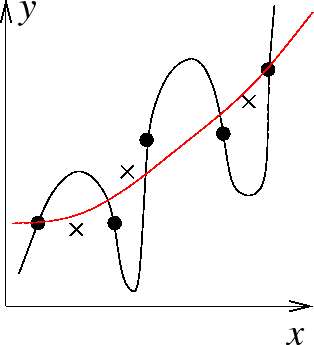
\includegraphics[width=0.8\textwidth]{overfitting.png}
\caption{\label{fig:OverfittingExample}Overfitting example, left one has a decent generalization performance and right one is overfitting.}
\end{figure}
From the example in Figure \ref{fig:OverfittingExample}, it is clear that a model, whose complexity is neither too small nor too large, has the best generalization performance. 

In order to find the optimal complexity of the neural network, there are mainly two approaches. One is to change the adaptive parameters, like neuron numbers in hidden layers. This is named structural stabilization. It can be approached from two directions. We can start from a small network and increasing layer number or neuron number in the learning process and arrive at a effective neural network architecture. The other one is to start from a large network and prune out layers or neurons in the learning process to achieve the optimal network. Another fundamental basis method to control the complexity of the model is use of regularization which includes add a penalty term in error function. The degree of regularization can be adjusted by scaling the term via a multiplicative parameter.

Regularization helps to smooth decision boundary surface via introducing a penalty term $\Omega$ to the error function
\begin{equation}\label{eq:Regularization}
\hat{E} = E + \lambda\Omega
\end{equation}
where $E$ is the standard error function and the $\lambda$ adjust the extent of the penalty $\Omega$ effects on the solution. The task of the learning is to minimize the total error function $\hat{E}$. It needs to compute the derivatives of $\Omega$ with respect to the weights efficiently. A model, which has high accuracy in training dataset, has a small value for $E$. At the same time, the smooth error surface of neural network give a small value for $\Omega$.

A number form of regularizers have been performed in practices, like weight decay, early stopping, training with noise, weight sharing etc..

\subsection{Weight Decay}

In order to make decision boundary surface smooth, the weight values should be small. The weight decay regularizer can be represented as
\begin{equation}\label{eq:WeightDcay}
\Omega = \frac{1}{2} \sum_i w_{i}^2
\end{equation}
where the sum includes all weights and biases. Weight decay of this form lead to major improvements in generalization empirically \citep{hinton1987learning}. Intuitively, in equation \ref{eq:WeightDcay}, the smaller the weightw are, the better the regularizer is. Usually, the derivatives of the total error function with respect to the weight is used to train neural network. The network is trained by gradient descent in the continuous time limit. The weights will evolve with time $t$
\begin{equation}\label{eq:WeightDecayTime}
\frac{w}{t} = -\eta\nabla E = -\eta\lambda w
\end{equation}
where $\eta$ is learning rate. And the equation has solution
\begin{equation}\label{eq:WeightDecaySolution}
w(t) = w(0)exp(-\eta\lambda t)
\end{equation}
and the exponential function reduce weights to zero quickly. Weight decay is also named L2 regularization.

\subsection{Dropout}

Neural network with deep layers and large amount of neurons is a very powerful learning machine. However, the more parameters the network has, the easier it is overfitting. Recently, dropout\citep{srivastava2014dropout} is a simple and extremely effective regularization technique which complements the other methods. At training stage, random neurons are selected with some probability $p$ to update their associated weights, and the others are inactive. In the other words, only a reduced network is trained based on the input data at the training stage. 
\graphicspath{ {./Figures/} }
\begin{figure}[!htb]
\centering
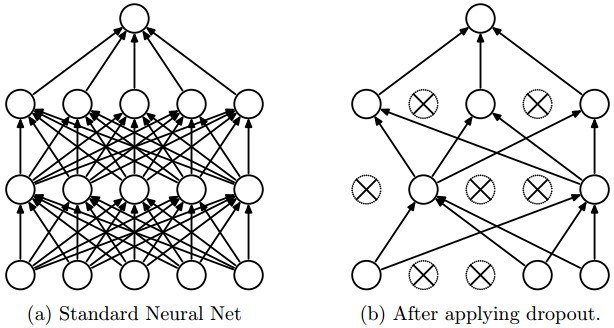
\includegraphics[width=0.8\textwidth]{dropout.jpeg}
\caption{\label{fig:Dropout}Illustration of dropout \citep{srivastava2014dropout}.}
\end{figure}
At testing stage, there is no dropout applied and all neurons are active. Dropout method is replaced by performing a scaling of layer outputs by the same probability $p$. This method can keep the outputs of neurons to be the same in both training and testing stages. For example, if a neuron has $p$ probability to be dropout in the training stage, the neuron should output $l$ without dropout in testing stage. Then we should apply $p\ast l + (1 - p)\ast 0)$ on the output, because the output has $(1-p)$ probability to be $0$.

\section{Softmax classifier}

Softmax function, also named normalized exponential, is a generalization of logistic function which squeezes a $d$ dimensional arbitrary real values vector to a $d$ dimensional vector of real values in the range $(0,1)$ that add up to 1. Because the softmax function is the gradient log normalizer of categorical probability distribution, it can be used in probabilistic multiclass classification methods.

The softmax function derives from log linear models and interprets the weights in terms of convenient odds ratios. We can constrain the layer input to the output neurons to be positive and divide by the sum.

The softmax layer begins the same way as normal layer which forms the weighted inputs $z^L_j = \sum_{k} w^L_{jk} x^{L-1}_k + b^L_j$ where $L$ is layer number, $k$ is input data number and $j$ is output neuron number. Then it implements a softmax function to the $z^L_j$ and the activation $a^L_j$ of the $j$ output neuron is
\begin{equation}\label{eq:SoftmaxActivation}
f_j(z) = \frac{e^{z_j}}{\sum_k e^{z_k}}
\end{equation}
The equation \ref{eq:SoftmaxActivation} implies that the output values are all positive and the sum of all values $\sum_k a_k$ is $1$.

Softmax classifier is used to handle a multiclass classification. For a training dataset $(x_{1}, y_{1}), \ldots, (x_{m}, y_{m}), y_{i} \in \{1, 2, \ldots, K\} $ of $m$ labelled examples, label $y$ can have $K$ different values.

Suppose to predict an unseen sample $x$, we will use hypothesis to estimate the probability $P(y=k | x)$ for each value $k = 1, \ldots, K$. For example, we want to compute the probability of the class label on each of $K$ different possible values. Then the neural network will output a $K$ dimensional vectors which represent $K$ estimated probabilities. 
%\begin{equation}\label{eq:SoftmaxPostPro}
\begin{align}
h_{W}(x) =
\begin{bmatrix}
P(y = 1 | x; W) \\
P(y = 2 | x; W) \\
\vdots \\
P(y = K | x; W)
\end{bmatrix}
=
\frac{1}{ \sum_{j=1}^{K}{\exp(W^{(j)\top} x) }}
\begin{bmatrix}
\exp(W^{(1)\top} x ) \\
\exp(W^{(2)\top} x ) \\
\vdots \\
\exp(W^{(K)\top} x ) \\
\end{bmatrix}
\end{align}
%\end{equation}
Where $W^{j}$ are the weights of the model and the normalized distribution ensures that the sum is one.

On the one hand, cross entropy can be used to interpreted softmax classifier. The cross entropy between actual  distribution $p$ and a predicted distribution $q$ is represented as
\begin{equation}\label{eq:CrossEntropyDiff}
H(p,q) = - \sum_x p(x) \log q(x)
\end{equation}
Hence, the task of softmax classifier is to minimize the cross entropy between the actual distribution and the predicted distribution. 

On the other hand, softmax classifier can be interpreted in probability view. Given a sample $(x_i, y_i)$ and parameters $W$, we can compute the normalized probability by
\begin{equation}\label{eq:ProbInter}
P(y_i \mid x_i; W) = \frac{e^{f_{y_i}}}{\sum_j e^{f_j} }
\end{equation}
where $f_{y_i}$ is the score predicted by the model with weights $W$. Therefore the normalized probabilities are computed by exponentiating the values and dividing sum of all values. Then we can minimize the negative log likelihood of the ground truth labels which can be regarded as performing Max Likelihood Estimation(MLE). Instead of MLE, Maximum a posteriori(MAP) can be used to evaluate the performance of the model.

\subsection{Practical issues}

For numerical view, the exponentiation computation is easy overflow. Thus, the output of softmax function is not numeric stable through computing $e^{f_{y_i}}$ and $\sum_j e^{f_{y_j}}$ in straight way. It is important to implement with a normalization trick. It is mathematically equivalent if multiplying a constant $C$ both with top and bottom of the fraction.
\begin{equation}\label{eq:SoftmaxTricks}
\frac{e^{f_{y_i}}}{\sum_j e^{f_j}}
= \frac{Ce^{f_{y_i}}}{C\sum_j e^{f_j}}
= \frac{e^{f_{y_i} + \log C}}{\sum_j e^{f_j + \log C}}
\end{equation}
where $C$ can be any positive value. The $C$ does not change the output value, while it can improve the numerical stability of the computation. An experienced choice of $C$ is to set $\log C = -\max_j f_j$, and it can shift the vector $f$ to preserve the highest value as $0$.

\subsection{Error function}
The error function is used to evaluate the performance of the model. We will generate an error function for softmax regression. An indicator function, $I\{\cdot\}$, is introduced to represent the accuracy for each label. If the predicted result corresponds to the actual label, say $y^{(i)} = k$, the indicator function returns $1$, otherwise $0$. The error function will be defined as
\begin{equation}\label{eq:LogLossFunc}
L(W) = - \left[ \sum_{i=1}^{m} \sum_{k=1}^{K}  I\left\{y^{(i)} = k\right\} \log \frac{\exp(W^{(k)\top} x^{(i)})}{\sum_{j=1}^K \exp(W^{(j)\top} x^{(i)})}\right]
\end{equation}
where this generates the logistic regression error function
\begin{align}\label{eq:LogRegLossFunc}
L(W) &= - \left[ \sum_{i=1}^m   (1-y^{(i)}) \log (1-h_W(x^{(i)})) + y^{(i)} \log h_W(x^{(i)}) \right] \\
&= - \left[ \sum_{i=1}^{m} \sum_{k=0}^{1} 1\left\{y^{(i)} = k\right\} \log P(y^{(i)} = k | x^{(i)} ; W) \right]
\end{align}
Similar to the logistic regression error function, the softmax error function sum over the predicted different $K$ values of the class value. In the softmax regression, the posterior probability distribution can be represented as
\begin{equation}\label{eq:PostProbDis}
P(y^{(i)} = k | x^{(i)} ; W) = \frac{\exp(W^{(k)\top} x^{(i)})}{\sum_{j=1}^K \exp(W^{(j)\top} x^{(i)}) }
\end{equation}
It is not easy to solve equation \ref{eq:LogRegLossFunc}. Usually an optimization algorithm can help to approximate the optimal value. Taking derivative with respect to weights, we can get the entire gradient 
\begin{equation}\label{eq:PartDer}
\nabla_{W^{(k)}} L(W) = - \sum_{i=1}^{m}{ \left[ x^{(i)} \left( 1\{ y^{(i)} = k\}  - P(y^{(i)} = k | x^{(i)}; W) \right) \right]  }
\end{equation}
We can take partial derivative of $L(W)$ with respect to the $j$th element of $W^{(k)}$.

\section{Convolutional Neural Networks}

Convolutional Neural Networks\citep{lecun1998gradient} (CNN) are widely applied in image understanding and achieve top rank in image classification competetion\citep{krizhevsky2012imagenet}. Compared to regular neural networks, CNN architectures assume that the inputs are images and pixels are related in region. Regular neural networks fully connect layers and the method is computation expensive.

CNN architecture have neurons arranged in 3 dimension, say width, height and depth. For example, there is an image which has dimensions $32x32x3$. The neurons in a layer will connect to a customised region of the previous layer. Moreover, the final output layer has dimensions $1x1xd$, where $d$ is the number of class. The dimensions are reduced from $3072$ to $d$. The output is a single vector of class scores.

\graphicspath{ {./Figures/} }
\begin{figure}[!htb]
\centering
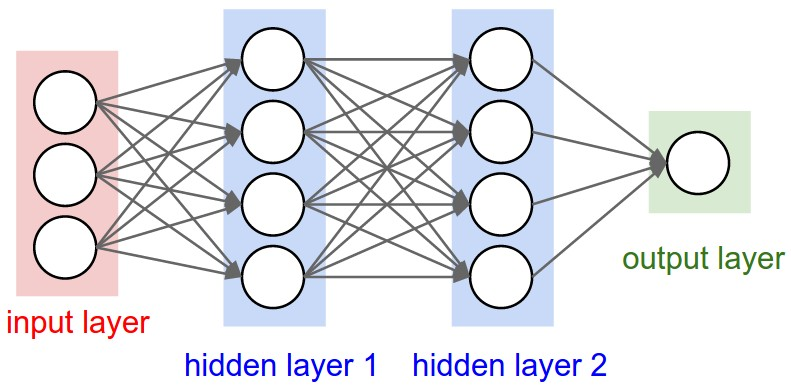
\includegraphics[width=0.4\textwidth]{neural_net2.jpeg}
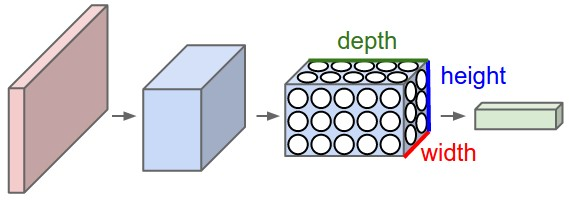
\includegraphics[width=0.4\textwidth]{cnn.jpeg}
\caption{\label{fig:perceptron}Left is a fully connect regular neural network. Right is a CNN in 3 dimensions.}
\end{figure}

\subsection{Layers in CNN}
CNNs have three main type of layers, convolutional layer, pooling layer and fully connected layer. Every layer transforms input to output via a differentiable function. 
\begin{enumerate}
  \item Convolutional layer compute the output of neurons which connect to local regions in previous layer. In brief, CNN apply a dot product between the weights and region in the input volume connected in the input. Dimensions have no change.
  \item ReLU layer acts as an activation function after convolutional layer. It leaves the dimensions unchanged. There is no parameters in ReLU layer.
  \item Pooling layer will downsample the input spatial dimensions(width, height). There is no parameters in pooling layer.
  \item Fully connected layer computes the output of neurons which connect all the neurons in the previous layer.
\end{enumerate}
Following layer by layer, CNN transforms an image from a set of pixel values to the final class scores.
 
\section{Spatial Pyramid Match}

Spatial pyramid match\citep{lazebnik2006beyond} is used to classify high-level semantic attributes, based on low-level features. The method subdivides a image in several different levels of resolution and counts features falling in each spatial bin. It extends bags of features and derives spatial information from images.
\graphicspath{ {./Figures/} }
\begin{figure}[!htb]
\centering
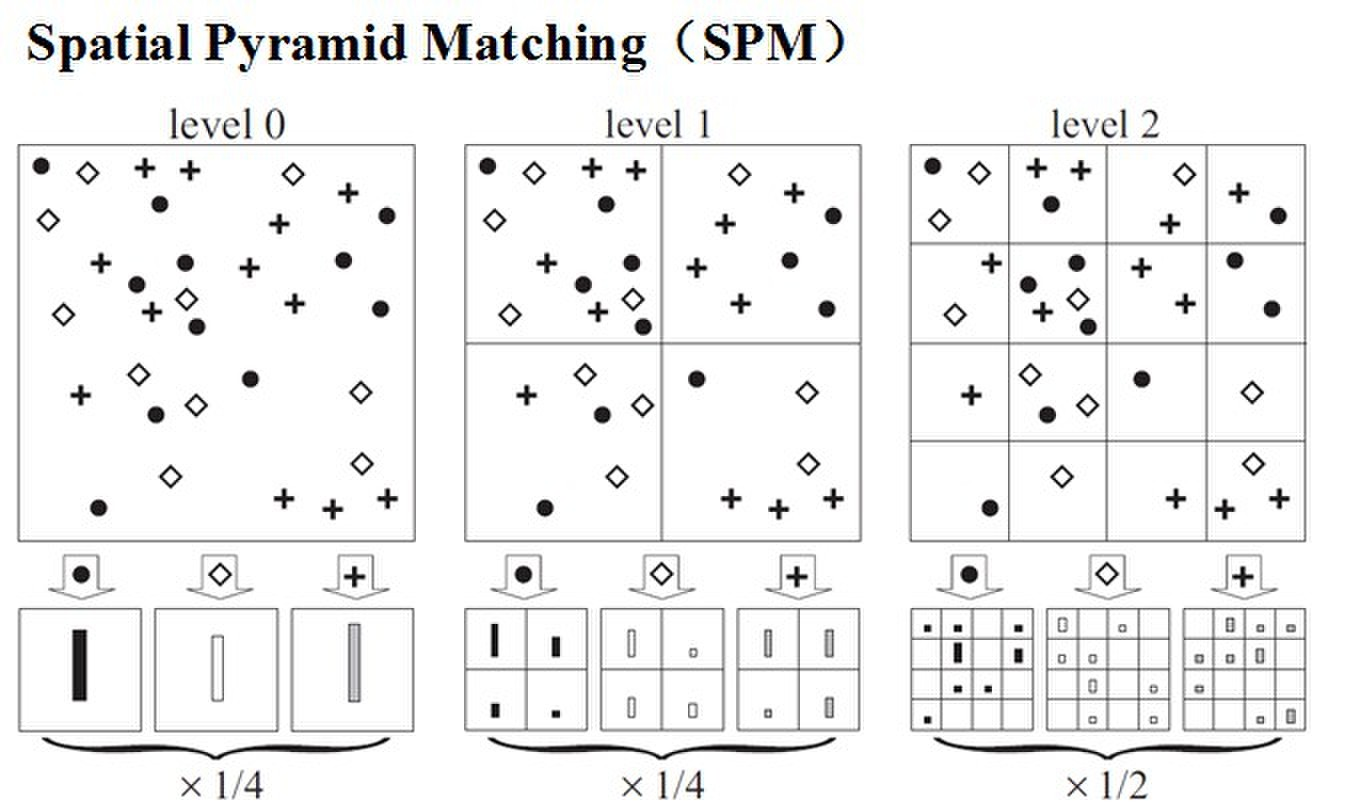
\includegraphics[width=0.8\textwidth]{spm.jpg}
\caption{\label{fig:perceptron}Diagram of Spatial Pyramid Match.}
\end{figure}

\section{Transfer Learning}

In machine learning literature, transfer learning\citep{pan2010survey} focuses on storing knowledge from one domain and applying it to a related problem. It has two benefits. One is saving time to build a model from scratch up. Another is saving effort to collect training data.

A domain with two components, a feature space and a marginal probability distribution, can be represented
\begin{equation}\label{eq:TransLearning}
D = \{ \chi, P(X) \}
\end{equation}
where $\chi$ is feature space and $P(X)$ is the marginal probability distribution. 
\graphicspath{ {./Figures/} }
\begin{figure}[!htb]
\centering
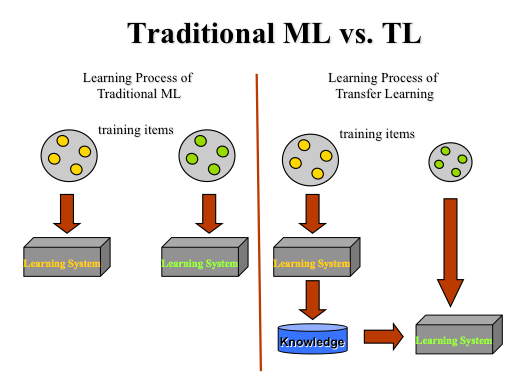
\includegraphics[width=0.8\textwidth]{MLvsTL.png}
\caption{\label{fig:perceptron}Diagram of Transfer Learning.}
\end{figure}
